\newpage
\section*{Обзор методов решения уравнения рендеринга} 

\subsection*{Алгоритм излучательности (radiosity)}
Рассмотрим частный случай уравнения рендеринга для диффузных материалов. Двулучевая функция отражения в этом случае представляет собой константу и уравнение сводится к тривиальному.
\begin{gather}
  J_{out}(x,y,z,\vec \omega) = J_{emit}(x,y,z,\vec \omega) + \int \limits_\Omega J_{in}(x,y,z,\vec \theta) \cdot f(x,y,z,\vec \omega,\vec \theta) \cdot \left\langle  {-\vec \theta \cdot \vec n} \right\rangle \cdot d\theta,
\end{gather}
где $J_{emit}$ -- излученная мощность точкой. Как мы уже упоминали, для диффузных материалов, значения ДФО не зависят ни от входящих, ни от исходящих направлений
\begin{gather}
  f(x,y,z,\vec \omega,\vec \theta) = \frac{\eta (x,y,z)}{\pi}
\end{gather}

\begin{gather}  
  \pi \cdot J_{out} = \pi \cdot J_{emit} + \eta \cdot \int_\Omega J_{in}(x,y,z,\vec \theta) \cdot \left\langle  {-\vec \theta \cdot \vec n} \right\rangle \cdot d\theta
\end{gather}

Далее, преобразуя интеграл по телесному углу в интеграл по всем точкам поверхности сцены, а также разбивая поверхность на непересекающиеся полигоны с постоянной излучательностью, в конечном итоге, получаем следующую систему линейных уравнений
\begin{gather}  
  B_i = E_i + \eta_i \cdot \sum_j F_{ij} B_j ,
\end{gather}
где $ B_i $ -- результирующая излучательность полигона, $ E_i $ -- излучаемая энергия полигоном, $ \eta_i $ -- коэффициент отражения, $ F_{ij} $ -- форм-фактор. 

Подробнее с преобразованиями и самой реализации метода можно ознакомиться здесь \cite{history}.

Минус данного метода в том, что он позволяет моделировать, в принципе, конкретный тип материала -- диффузный. В реальной жизни, как уже упоминалось, это встречается не всегда.

\subsection*{Алгоритм <<бросания лучей>> ray-casting}

Фактически, данный метод учитывает только первично-освещенные точки поверхности, а значит он также помогает произвести расчет теней. Из точки выпускается луч по направлению к источнику. Если этот луч имеет пересечения с каким-либо фрагментом поверхности, то значит, что точка, из которой был выпущен луч, находится в тени. В ином случае, рассчитываем долю энергии получаемую точкой \cite{history}.

\begin{center}
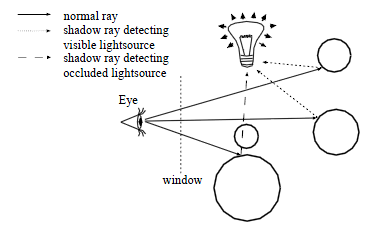
\includegraphics[width=0.5\linewidth]{ray-casting.png}
\end{center}

\subsection*{Алгоритм visibility ray-tracing и трассировка фотонов}

Предыдущий алгоритм учитывал только первично-освещенные точки. Повысив дальность прохода лучей, то есть увеличив количество отражений и преломлений получим более точную модель. Различия visibility ray-tracing и трассировки фотонов лишь в направлении (от источника или же к источнику). 

\begin{center}
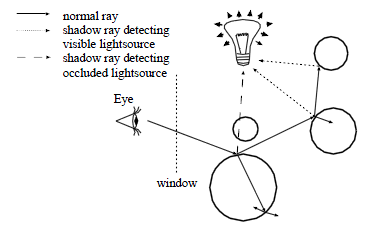
\includegraphics[width=0.5\linewidth]{ray-tracing.png}
\end{center}

\subsection*{Метод Монте-Карло (на базе трассировки лучей) и стохастические методы}

Все пространство разбивается равномерной сеткой. Количество узлов в трехмерном пространстве при этом равно $N^3$. Узлы, по которым ведется интегрирование, выбираются случайно. Соответственно, при увеличении числа узлов интеграл, вычисленный методом Монте-Карло  \cite{history}, приближается к точному значению. Но при недостаточном количестве узлов получаем шумы. Шумы убираются размытием. 

\subsection*{Гибридные алгоритмы}

Каждый из приведенных выше алгоритмов обладает своими сильными и слабыми сторонами. Так алгоритм излучательности позволяет быстро рассчитать освещенность, но только для диффузных поверхностей. С другой стороны, алгоритм трассировки лучей имеет в своих недостатках низкую скорость, но является более универсальным. На этой основе появляется гибридные многопроходные алгоритмы, в которых расчет делится на несколько независимых этапов. Так, использование только алгоритма излучательности позволяет рассчитывать взаимодействие и взаимовлияние диффузных поверхностей в пространстве, трассировка же учитывает зеркальную составляющую. Характерным примером данной группы алгоритмов являются алгоритмы Сллиона, Ширли, Чена  \cite{history}.

